\chapter{Arhitektura i dizajn sustava}
		
		\section{Baza podataka}
			
		\
		Za potrebe našeg sustava koristit ćemo relacijsku bazu podataka koja olakšava svojom strukturom modeliranje stvarnog svijeta. Gradivna jedinka baze je relacija, odnosno tablica koja je definirana svojim imenom i skupom atributa. Zadaća baze podataka je brza i jednostavna pohrana, izmjena i dohvat podataka za daljnju obradu. Za upravitelja baze podataka odabrali smo Postgresql.
        Baza podataka ove aplikacije sastoji se od sljedecih entiteta: 
        
        \begin{packed_item}
						\item Registrirani
						\item Moderator
						\item Oglas
						\item Replies
						\item Grade
						\item DeletedOglas
						\item Category
						\item Course
						\item Study Programme
		\end{packed_item}
		
			\subsection{Opis tablica}
			
				\noindent\textbf{Registirani} \ Ovaj entitet sadržava sve važne informacije o registriranom korisniku aplikacije. Sadrži atribute: userID, firstName, lastName, userName, userAvatar, password, email i created. Ovaj entitet je generalizacija entiteta Moderator. Ovaj entitet u vezi je \textit{1:N} s entitetom Oglas preko userID, u vezi je \textit{1:N} s entitetom Replies preko userID i u dvosturkoj vezi je \textit{0..1:N} s entitetom Grade preko userID-a. 
				
				\begin{longtblr}[
					label=none,
					entry=none
					]{
						width = \textwidth,
						colspec={|X[6,l]|X[6, l]|X[20, l]|}, 
						rowhead = 1,
					} 
					\hline 
					\multicolumn{3}{| c |}{\textbf{Registrirani}}	 \\ \hline[3pt]
					\SetCell{LightGreen}userID & INT	&  jedinstveni identifikator korisnika
					\\ \hline
					FirstName	& VARCHAR & ime korisnika  	\\ \hline 
					LastName & VARCHAR & prezime korisnika   \\ \hline 
					UserName & VARCHAR	& korisničko ime korisnika 		\\ \hline 
					UserAvatar & VARCHAR & profilna slika korisničkog računa  	\\ \hline 
					Password & VARCHAR & hash lozinke  	\\ \hline
					Email & VARCHAR & email adresa korisnika  	\\ \hline
					Created & DATE & datum stvaranja korisničkog računa  	\\ \hline 
				\end{longtblr}
				
				\noindent\textbf{Moderator} \ Ovaj entitet je specijalizacija entiteta Registrirani. Entitet je namijenjen korisnicima koji imaju ulogu moderatora i njegove funkcionalnosti. Sadrži atribut userID. Ovaj entitet u vezi je \textit{1:N} s entitetom DeletedOglas preko korisničkog ID-a(userID).
				
				\begin{longtblr}[
					label=none,
					entry=none
					]{
						width = \textwidth,
						colspec={|X[6,l]|X[6, l]|X[20, l]|}, 
						rowhead = 1,
					} 
					\hline 
					\multicolumn{3}{| c |}{\textbf{Moderator}}	 \\ \hline[3pt]
					\SetCell{LightGreen}userID & INT	&  jedinstveni identifikator korisnika
					\\ \hline
				\end{longtblr}
				
				\noindent\textbf{DeletedOglas} \ Ovaj entitet sadržava informacije o moderatoru aplikacije i oglasu koji je taj moderator izbrisao uz dano objašnjenje. Sadrži atribute: oglasID, deletorUserID i explanation. Ovaj entitet u vezi je \textit{1:N} s entitetom Oglas preko oglasID-a.
				
				\begin{longtblr}[
					label=none,
					entry=none
					]{
						width = \textwidth,
						colspec={|X[6,l]|X[6, l]|X[20, l]|}, 
						rowhead = 1,
					} 
					\hline 
					\multicolumn{3}{| c |}{\textbf{DeletedOglas}}	 \\ \hline[3pt]
					\SetCell{LightGreen}oglasID & INT	&  jedinstveni identifikator oglasa
					\\ \hline
					\SetCell{LightBlue}deletorUserID	& INT & jedinstveni identifikator moderatora  	\\ \hline 
					explanation & VARCHAR & objašnjenje brisanja oglasa   \\ \hline 
				\end{longtblr}
				
				\noindent\textbf{Oglas} \ Ovaj entitet je identifikacijski slab entitet kojeg entitet Registrirani identificira. Ovaj entitet sadržava sve važne informacije o objavljenom oglasu. Sadrži atribute: oglasID, oglasTitle, oglasDescription, timeOfCreation, vrstaOglasa, creatorUserID i idKategorije. Ovaj entitet u vezi je \textit{1:N} s entitetom Replies preko oglasID-a,u vezi je \textit{N:1} s entitetom Category preko idKategorije, u vezi je \textit{0..1:N} s entitetom Grade preko oglasID-a, u vezi je \textit{1:N} s entitetom DeletedOglas preko oglasID-a i u vezi je \textit{N:1} s entitetom Registrirani preko userID-a.
				
				\begin{longtblr}[
					label=none,
					entry=none
					]{
						width = \textwidth,
						colspec={|X[10,l]|X[6, l]|X[20, l]|}, 
						rowhead = 1,
					} 
					\hline 
					\multicolumn{3}{| c |}{\textbf{Oglas}}	 \\ \hline[3pt]
					\SetCell{LightGreen}oglasID & INT	&  jedinstveni identifikator oglasa
					\\ \hline
					oglasTitle	& VARCHAR & naslov oglasa  	\\ \hline 
					oglasDescription & VARCHAR & opis oglasa   \\ \hline 
					timeOfCreation & DATE	& vrijeme kreiranja oglasa 		\\ \hline 
					vrstaOglasa & VARCHAR & kategorija oglasa(nudim ili tražim)  	\\ \hline 
					\SetCell{LightBlue}creatorUserID & INT & jedinstveni identifikator kreatora oglasa  	\\ \hline
					\SetCell{LightBlue}idKategorije & INT & jedinstveni identifikator kategorije   	\\ \hline
				\end{longtblr}
				
				\noindent\textbf{Replies} \ Ovaj entitet je identifikacijski slab entitet kojeg entitet Registrirani identificira. Ovaj entitet sadržava sve važne informacije o odgovoru tj. upitu za oglas. Sadrži atribute: replyID, replyText, replyCreated, statusValue, replyCreatorID i oglasID. Ovaj entitet u vezi je \textit{N:1} s entitetom Oglas preko oglasID-a i u vezi je \textit{N:1} s entitetom Registrirani preko replyCreatorID-a.
				
				\begin{longtblr}[
					label=none,
					entry=none
					]{
						width = \textwidth,
						colspec={|X[10,l]|X[6, l]|X[20, l]|}, 
						rowhead = 1
					} 
					\hline 
					\multicolumn{3}{| c |}{\textbf{Replies}}	 \\ \hline[3pt]
					\SetCell{LightGreen}replyID & INT	&  jedinstveni identifikator upita
					\\ \hline
					replyText & VARCHAR & tekst upita  	\\ \hline 
					replyCreated & DATE & vrijeme kreiranja upita   \\ \hline 
					statusValue & VARCHAR	& status upita		\\ \hline 
					\SetCell{LightBlue}replyCreatorID & INT & jedinstveni identifikator kreatora upita  	\\ \hline
					\SetCell{LightBlue}oglasID & INT & jedinstveni identifikator oglasa   	\\ \hline
				
				\end{longtblr}
				
				\noindent\textbf{Grade} \ Ovaj entitet je identifikacijski slab entitet kojeg entitet Registrirani i entitet Oglas identificiraju. Ovaj entitet sadržava informacije o ocjeni studenta-pomagača. Sadrži atribute: instructorID, learnerID, oglasID i grade. Ovaj entitet u vezi je \textit{N:1} s entitetom Oglas preko oglasID-a i dvostruko je vezan \textit{N:1} s entitetom Registrirani preko instructorID-a i learnerID-a.
				
				\begin{longtblr}[
					label=none,
					entry=none
					]{
						width = \textwidth,
						colspec={|X[10,l]|X[6, l]|X[20, l]|}, 
						rowhead = 1
					} 
					\hline 
					\multicolumn{3}{| c |}{\textbf{Grade}}	 \\ \hline[3pt]
					\SetCell{LightGreen}instructorID & INT	&  jedinstveni identifikator studenta-pomagača
					\\ \hline
					\SetCell{LightGreen}learnerID & INT & jedinstveni identifikator studenta koji traži pomoć  	\\ \hline 
					\SetCell{LightGreen}oglasID & INT & jedinstveni identifikator oglasa   \\ \hline 
					ocjena & INT	& ocjena dana studentu-pomagaču za dane instrukcije		\\ \hline 

				
				\end{longtblr}
				
				\noindent\textbf{Category} \ Ovaj entitet sadržava informacije o kategoriji oglasa. Sadrži atribute: idKategorije, categoryName i courseID. Ovaj entitet u vezi je \textit{1:N} s entitetom Oglas preko idKategorije i u vezi je \textit{N:1} s entitetom Course preko courseID-a.
				
				\begin{longtblr}[
					label=none,
					entry=none
					]{
						width = \textwidth,
						colspec={|X[10,l]|X[6, l]|X[20, l]|}, 
						rowhead = 1
					} 
					\hline 
					\multicolumn{3}{| c |}{\textbf{Category}}	 \\ \hline[3pt]
					\SetCell{LightGreen}idKategorije & INT	&  jedinstveni identifikator kategorije(MI, blic, Ispitni rok)
					\\ \hline
					categoryName & VARCHAR & ime kategorije 	\\ \hline 
					\SetCell{LightBlue}courseID & INT & jedinstveni identifikator kolegija   \\ \hline

				
				\end{longtblr}
				

				
				\noindent\textbf{Course} \ Ovaj entitet sadržava informacije o kolegiju. Sadrži atribute: courseID, courseName i kraticaCourse i programmeID. Ovaj entitet u vezi je \textit{1:N} s entitetom Category preko idKategorije i u vezi je \textit{N:1} s entitetom Study Programme preko programmeID-a.
				
				\begin{longtblr}[
					label=none,
					entry=none
					]{
						width = \textwidth,
						colspec={|X[10,l]|X[6, l]|X[20, l]|}, 
						rowhead = 1
					} 
					\hline 
					\multicolumn{3}{| c |}{\textbf{Course}}	 \\ \hline[3pt]
					\SetCell{LightGreen}courseID & INT	&  jedinstveni identifikator kolegija
					\\ \hline
					courseName & VARCHAR & ime kolegija 	\\ \hline
					kraticaCourse & VARCHAR & kratica kolegija 	\\ \hline 
					\SetCell{LightBlue}programmeID & INT & jedinstveni identifikator smjera(E ili R)   \\ \hline
                

				\end{longtblr}
				
				
				\noindent\textbf{Study Programme} \ Ovaj entitet sadržava informacije o smjer kojem kolegij pripada. Sadrži atribute: programmeID i programmeName. Ovaj entitet u vezi je \textit{1:N} s entitetom Course preko programmeID-a.
				
				\begin{longtblr}[
					label=none,
					entry=none
					]{
						width = \textwidth,
						colspec={|X[10,l]|X[6, l]|X[20, l]|}, 
						rowhead = 1
					} 
					\hline 
					\multicolumn{3}{| c |}{\textbf{Study Programme}}	 \\ \hline[3pt]
					\SetCell{LightGreen}programmeID & INT	&  jedinstveni identifikator kolegija
					\\ \hline
					progammeName & VARCHAR & ime smjera 	\\ \hline
				\end{longtblr}
			
			\eject
			\subsection{Dijagram baze podataka}
			\begin{fig}
			    \graphicspath{ {slike/} }
  
                \centering
                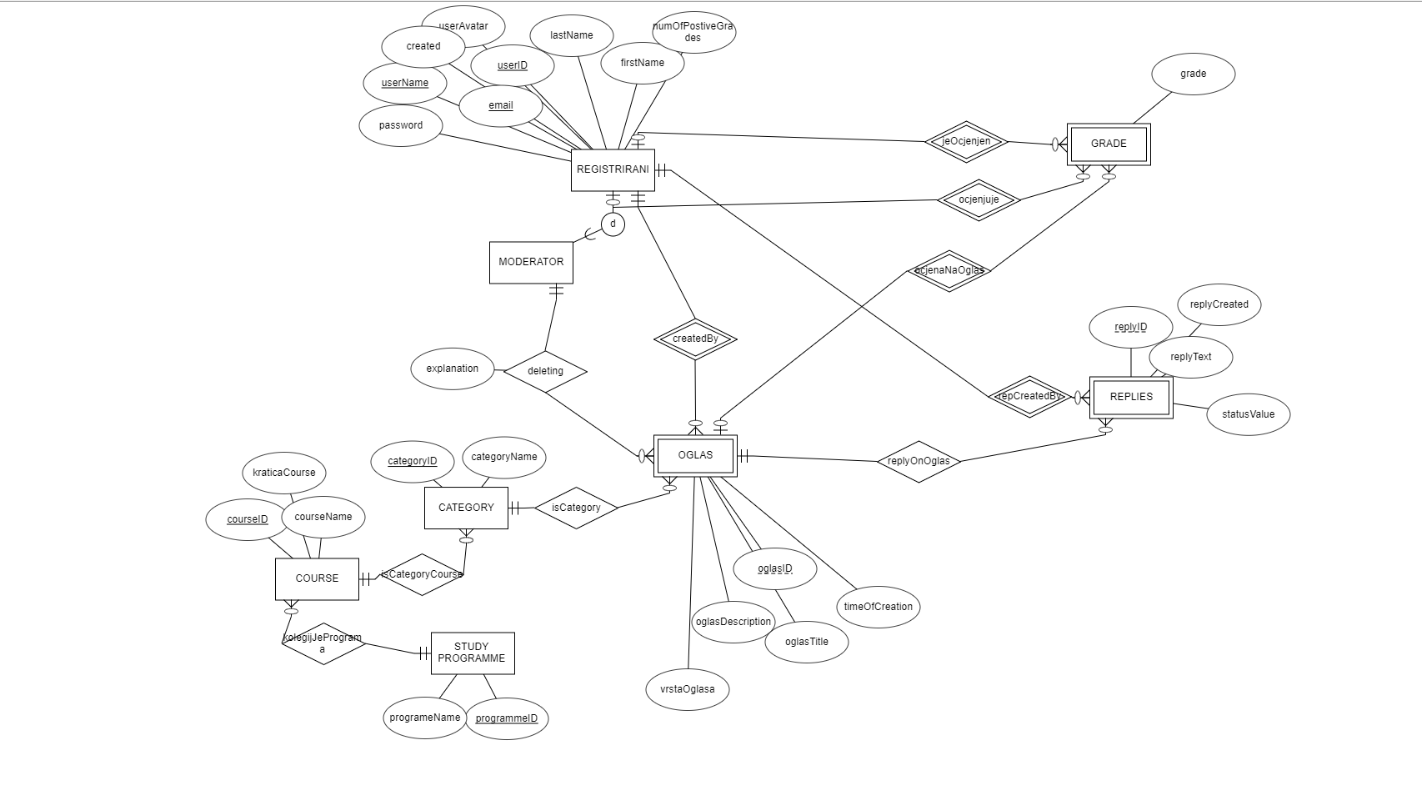
\includegraphics[width=\textwidth]{ER-dijagram Baze Podataka}
                \caption{\Slika 4.1: E-R dijagram baze podataka.}
			    
			\end{fig}

 
			
			\eject
			
			
		\section{Dijagram razreda}
		
			\textit{Potrebno je priložiti dijagram razreda s pripadajućim opisom. Zbog preglednosti je moguće dijagram razlomiti na više njih, ali moraju biti grupirani prema sličnim razinama apstrakcije i srodnim funkcionalnostima.}\\
			
			\textbf{\textit{dio 1. revizije}}\\
			
			\textit{Prilikom prve predaje projekta, potrebno je priložiti potpuno razrađen dijagram razreda vezan uz \textbf{generičku funkcionalnost} sustava. Ostale funkcionalnosti trebaju biti idejno razrađene u dijagramu sa sljedećim komponentama: nazivi razreda, nazivi metoda i vrste pristupa metodama (npr. javni, zaštićeni), nazivi atributa razreda, veze i odnosi između razreda.}\\
			
			\textbf{\textit{dio 2. revizije}}\\			
			
			\textit{Prilikom druge predaje projekta dijagram razreda i opisi moraju odgovarati stvarnom stanju implementacije}
			
			
			
			\eject
		
		\section{Dijagram stanja}
			
			
			\textbf{\textit{dio 2. revizije}}\\
			
			\textit{Potrebno je priložiti dijagram stanja i opisati ga. Dovoljan je jedan dijagram stanja koji prikazuje \textbf{značajan dio funkcionalnosti} sustava. Na primjer, stanja korisničkog sučelja i tijek korištenja neke ključne funkcionalnosti jesu značajan dio sustava, a registracija i prijava nisu. }
			
			
			\eject 
		
		\section{Dijagram aktivnosti}
			
			\textbf{\textit{dio 2. revizije}}\\
			
			 \textit{Potrebno je priložiti dijagram aktivnosti s pripadajućim opisom. Dijagram aktivnosti treba prikazivati značajan dio sustava.}
			
			\eject
		\section{Dijagram komponenti}
		
			\textbf{\textit{dio 2. revizije}}\\
		
			 \textit{Potrebno je priložiti dijagram komponenti s pripadajućim opisom. Dijagram komponenti treba prikazivati strukturu cijele aplikacije.}